\section*{Resultados e Discussão}

Ilustrações e gráficos devem ser apresentados com tamanho e detalhes suficientes para a composição gráfica final, preferivelmente na mesma posição do texto.

\textbf{Gráficos:} devem apresentar-se sem bordas, descritos com o mesmo tipo e tamanho de letras contidas no texto e a legenda na posição inferior do mesmo. A numeração deve ser sucessiva em algarismos arábicos.

\textbf{Tabelas:} evitar tabelas extensas e dados supérfluos; adequar seus tamanhos ao espaço útil do papel e colocar, na medida do possível, apenas linhas contínuas horizontais; suas legendas devem ser concisas e autoexplicativas. Na discussão, confrontar os dados obtidos com a literatura.
\vspace{0.5cm}

\noindent\textbf{Modelos de Figuras:}


\begin{figure}[ht]
\centering
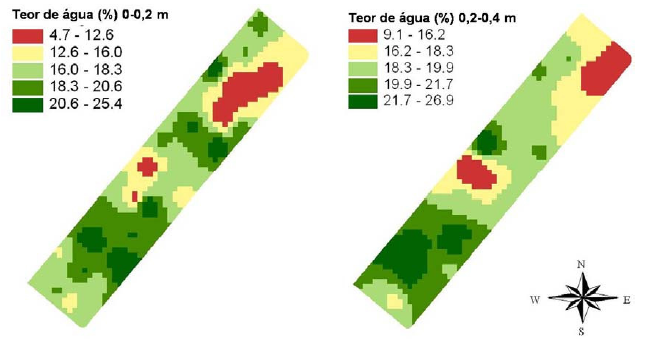
\includegraphics[width=10cm,angle=0]{imagens/grafico_1}
\caption{Mapas de teor de água das camadas de 0-2,2 e 0,2-0,4 m de profundidade.}
\label{fig:nome_referencia_figura1}
\end{figure}

\begin{figure}[ht]
\centering
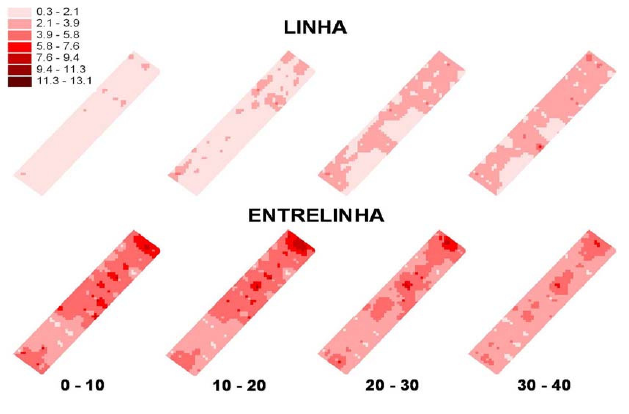
\includegraphics[width=10cm,angle=0]{imagens/grafico_2.png}
\caption{Mapas do índice de cone (MPa) referente aos dados coletados nas diferentes profundidades nas linhas e nas entrelinhas da cultura da cana.}
\label{fig:nome_referencia_figura2}
\end{figure}

\newpage
\noindent\textbf{Modelo de Tabela:}

\begin{table}[ht]
\caption{Análise do IC nas linhas (L) e entrelinhas (E) de cana nas diferentes profundidades amostradas pelo índice de cone.}
\vspace{.2cm}
\centering
\resizebox{\textwidth}{!}{%
\begin{tabular}{ccccccccc}
\hline
Profundidade (m) & \multicolumn{2}{c}{0 a 0,1} & \multicolumn{2}{c}{0,1 a 0,2} & \multicolumn{2}{c}{0,2 a 0,3} & \multicolumn{2}{c}{0,3 a 0,4} \\ \hline
                 & L            & E            & L             & E             & L             & E             & L             & E             \\
Média (MPa)      & 1,39**       & 4,28**       & 1,86**        & 4,29**        & 2,20**        & 3,83**        & 2,46**        & 3,44**        \\
CV(\%)           & 54           & 57           & 55            & 54            & 46            & 49            & 48            & 43            \\ \hline
\end{tabular}%
}
\small{**:valores significativos para o nível de significância de 1\% pelo teste de Tukey; L – linhas; E – entrelinhas.}
\label{tab:nome_tabela1}
\end{table}